\documentclass{article}

%
% 引入模板的style文件
%
\usepackage{homework}


%
% 封面
%

\title{
	
\includegraphics[scale = 0.45]{images/title/ucas-logo1.png}\\
    \vspace{1in}
    \textmd{\textbf{\hmwkClass\ \hmwkTitle}}\\
    \textmd{\textbf{\hmwkSubTitle}}\\
    \normalsize\vspace{0.1in}\small{\hmwkCompleteTime }\\
    \vspace{0.1in}\large{\textit{\hmwkClassInstructor\ }}\\
    \vspace{3in}
}

\author{\hmwkAuthorName \\ 
	\hmwkAuthorStuID}
\date{}

\renewcommand{\part}[1]{\textbf{\large Part \Alph{partCounter}}\stepcounter{partCounter}\\}


%
% 正文部分
%
\begin{document}


\maketitle


%\include{chapters/ch01}


\pagebreak

\begin{homeworkProblem}
\textbf{1.	选择的爬虫工具是什么?该工具具有什么特点?}\\
	\textbf{Solution:}\\
	{\color{blue}Scrapy框架是基于python的一个库,为了抓取网页数据、提取结构性数据而编写的应用框架,该框架是封装的,包含 request (异步调度和处理)、下载器(多线程的 Downloader)、解析器(selector)和 twisted(异步处理)等。对于网站的内容爬取,其速度非常快捷。优点:通过管道的方式存入数据库,灵活,可保存为多种形式。缺点:无法用它完成分布式爬取~\cite{tang2015extreme}。
MRR@20是准确推荐项目的排序倒数平均值,该指标衡量的是模型推荐项目的排序性能~\cite{li2017neural}。直观地说,在实践中推荐准确的项目排序得越高越好。MRR@20的定义如下:

\begin{center}
	\begin{eqnarray}
		\text{MRR}@20=\frac{1}{|\mathcal{T}|}\sum_{u \in \mathcal{T}}\frac{1}{{R_{u,g_u}}},
		\label{eq:MRR}
	\end{eqnarray}
\end{center}
其中,如果$R_{u,g_u}\geq 20$,排序的倒数值将设置为0。	
  
\begin{table}[htbp]
	\centering
	\caption{购买预测数据中冷启动用户的比例}
	\label{coldstartuser}
	\begin{tabular}{c|cc}
		\hline
		数据集 & \#冷启动用户  & 比例 (\%)   \\
		%Dataset & \#Cold-start Users  & Percentage (\%)   \\
		\hline
		$D_1$   & 225,749 & 52.34     \\
		$D_2$  & 245,703 & 60.96     \\
		$D_3$   & 121,006   & 55.61    \\
		\hline
	\end{tabular}%\vspace{-0.3cm}
\end{table}

}
\end{homeworkProblem}


\begin{homeworkProblem}
	\textbf{2.	爬虫工具环境部署成功截图。}\\
	\textbf{Solution:}\\
	\begin{figure}[H]  % 这里记得用[H]
		\centering
		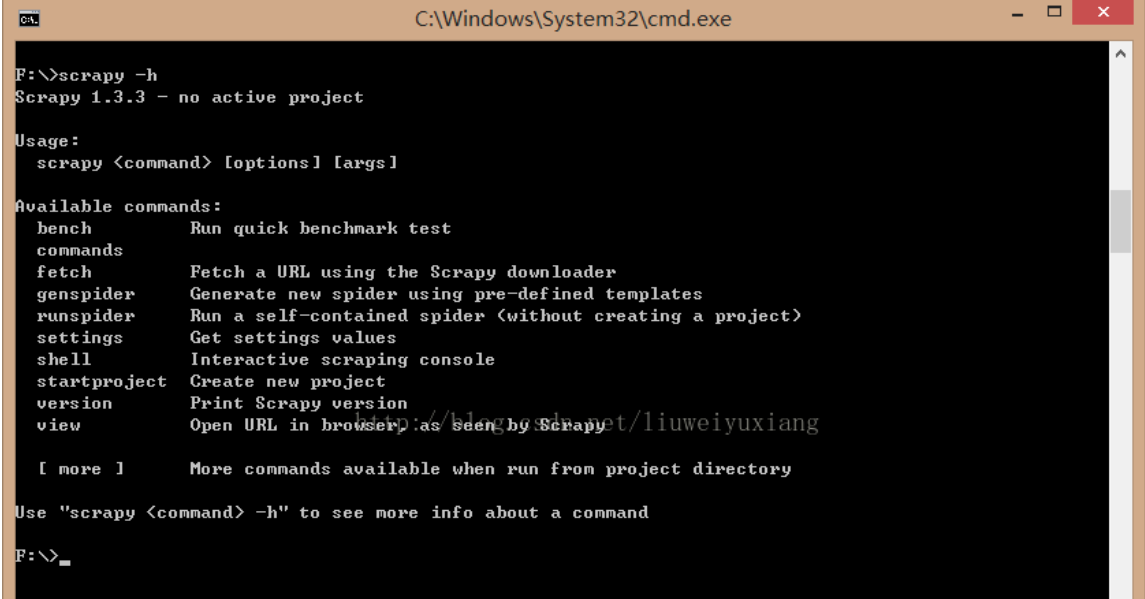
\includegraphics[width=0.7\linewidth]{images/Fig1}
		\caption{Scrapy环境部署成功}
		\label{fig:ucas-logo}
	\end{figure}
	
\end{homeworkProblem}


\pagebreak

\begin{homeworkProblem}
\textbf{3.	爬取豆瓣电影Top250页面~\cite{guo2019buying}, 开始的URL:https://movie.douban.com/top250,获取每部电影的序号、片名、导演、编剧、主演、类型、制作国家/地区、语言、上映日期、片长、又名、豆瓣评分和剧情简介等内容,将数据存入本地txt或者xlsx文件。}\\
\textbf{Solution:}\\
{\color{blue}

(1) 打开url并返回BeautifulSop对象: 
\begin{figure}[H]  % 这里记得用[H]
	\centering
	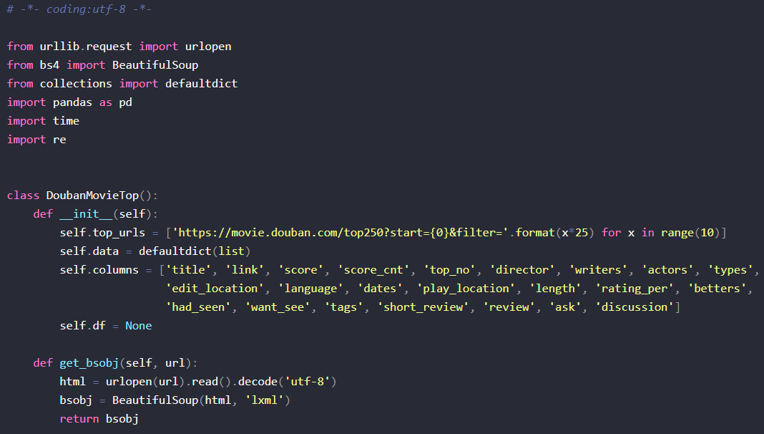
\includegraphics[width=0.75\linewidth]{images/Fig2}
	\caption{返回BeautifulSop对象}
	\label{fig:ucas-logo}
\end{figure}

(2) 解析并获取目标对象: 
\begin{figure}[H]  % 这里记得用[H]
	\centering
	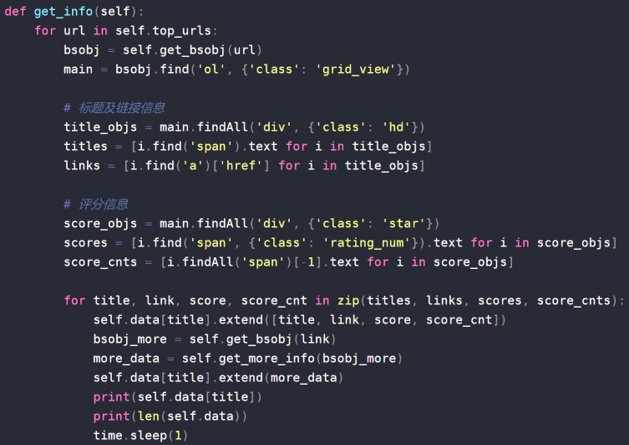
\includegraphics[width=0.75\linewidth]{images/Fig3}
	\caption{解析并获取目标对象}
	\label{fig:ucas-logo}
\end{figure}


(3) 爬虫数据存为csv格式文件 :
	\begin{figure}[H]  % 这里记得用[H]
		\centering
		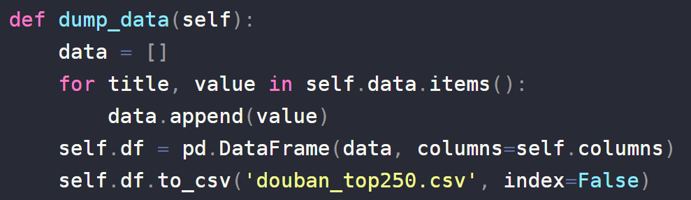
\includegraphics[width=0.7\linewidth]{images/Fig4}
		\caption{爬虫结果存储}
		\label{fig:ucas-logo}
	\end{figure}

(4)运行执行函数: 
	\begin{figure}[H]  % 这里记得用[H]
	\centering
	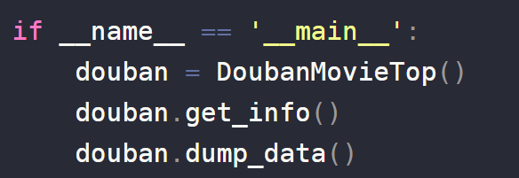
\includegraphics[width=0.7\linewidth]{images/Fig5}
	\caption{爬虫执行的主函数}
	\label{fig:ucas-logo}
\end{figure}


(5)爬虫结果展示:
	\begin{figure}[H]  % 这里记得用[H]
	\centering
	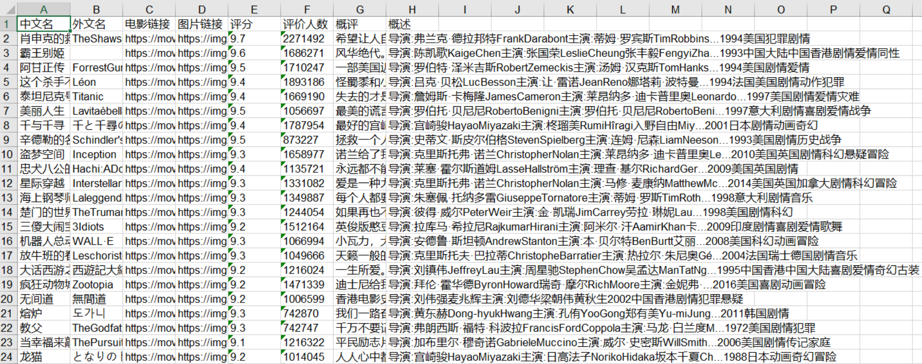
\includegraphics[width=1\linewidth]{images/Fig6}
	\caption{CSV保存的爬虫数据}
	\label{fig:ucas-logo}
\end{figure}
}


\end{homeworkProblem}
\pagebreak

\begin{homeworkProblem}
\textbf{4.附加题:在上述的爬虫程序中将获取的数据直接传入数据库,选择的什么数据库,导入数据的代码的截图和最终数据查询的截图。}\\
\textbf{Solution:}\\
{\color{blue}
空
}
\end{homeworkProblem}


% 引用文献
\bibliographystyle{unsrt}  % unsrt:根据引用顺序编号
\bibliography{refs}


\end{document}
